\documentclass{article}
\usepackage[utf8]{inputenc}
\usepackage{graphicx}
\usepackage{epstopdf}
\usepackage{float}
\usepackage[margin=1.25in]{geometry}
\usepackage{amsmath}
\usepackage{amssymb}
\usepackage{color} 
\usepackage{fancyvrb} 
\newcommand{\Vg}{{$V_{G}$}}
\newcommand{\Vsb}{{$V_{SB}$}}
\newcommand{\Vgb}{{$V_{GB}$}}
\newcommand{\Vds}{{$V_{DS}$}}
\newcommand{\Vs}{{$V_{S}$}}
\newcommand{\Vbs}{{$V_{BS}$}}
\newcommand{\Vb}{{$V_{b}$}}
\newcommand{\Va}{{$V_{A}$}}
\newcommand{\Vtwo}{{$V_{2}$}}
\newcommand{\Vone}{{$V_{1}$}}
\newcommand{\gdm}{{$G_{dm}$}}
\newcommand{\Vd}{{$V_{D}$}}
\newcommand{\Vdd}{{$V_{dd}$}}
\newcommand{\If}{{$I_{F}$}}
\newcommand{\Ir}{{$I_{R}$}}
\newcommand{\Iin}{{$I_{in}$}}
\newcommand{\Iout}{{$I_{out}$}}
\newcommand{\Vt}{{$V_{T0}$}}
\newcommand{\Ut}{{$U_T$}}
\newcommand{\Is}{{$I_{s}$}}
\newcommand{\Isat}{{$I_{sat}$}}
\newcommand{\gm}{{$g_{m}$}}
\newcommand{\gmro}{{$g_{m}r_{o}$}}
\newcommand{\gs}{{$g_{s}c$}}
\newcommand{\ro}{{$r_{o}$}}
\newcommand{\Vdm}{{$V_{dm}$}}
\newcommand{\Vdssat}{{$V_{DSSat}$}}
\newcommand{\Vsdsat}{{$V_{SDSat}$}}
\newcommand{\nMOS}{{\textit{n}MOS }}
\newcommand{\pMOS}{{\textit{p}MOS }}
\title{Circuits Lab 7}
\author{Cory Dolphin and Noam Rubin}
\date{April 3, 2013}

\begin{document}

\maketitle

\section*{Current as a function of voltage}
\begin{figure}[H]
\centering
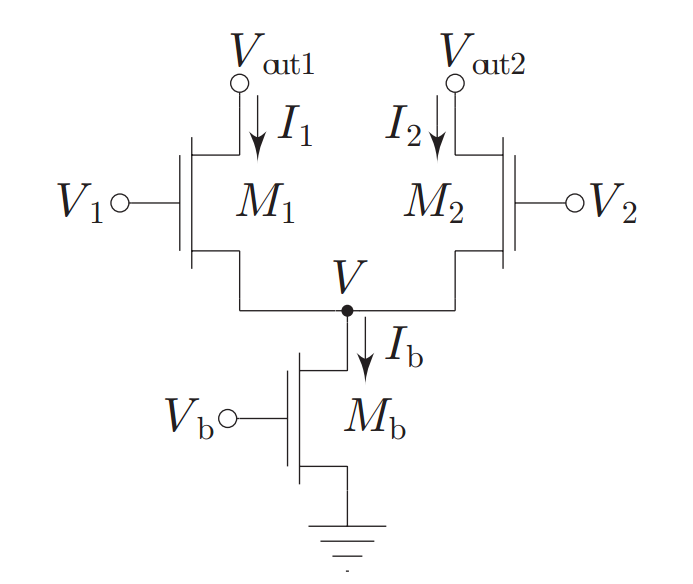
\includegraphics[width=0.65\linewidth]{./Figures/Schematic.png}
\caption{The differential pair circuit used in this experiment.}
\label{fig:Schematic}
\end{figure}

In this experiment, we constructed an \nMOS differential pair, as shown in Figure \ref{fig:Schematic}. We set the bias voltage, \Vb, to $0.5V$, and set $V_2$ to a range of voltages, from $1V$ to $4.5V$, sweeping $V_{DM}$ from $-30mV$ to $+30mV$. Each of these three data series, with $I_1$, $I_2$, $I_1 - I_2$ and $I_1 + I_2$ can be seen plotted on one figure, in Figure \ref{fig:AllCurrentsOneFigure}. Meanwhile, because of the large number of data series requested, we created four subplots containing the same information, which we will use for the purpose of analysis.
\begin{figure}[H]
\centering
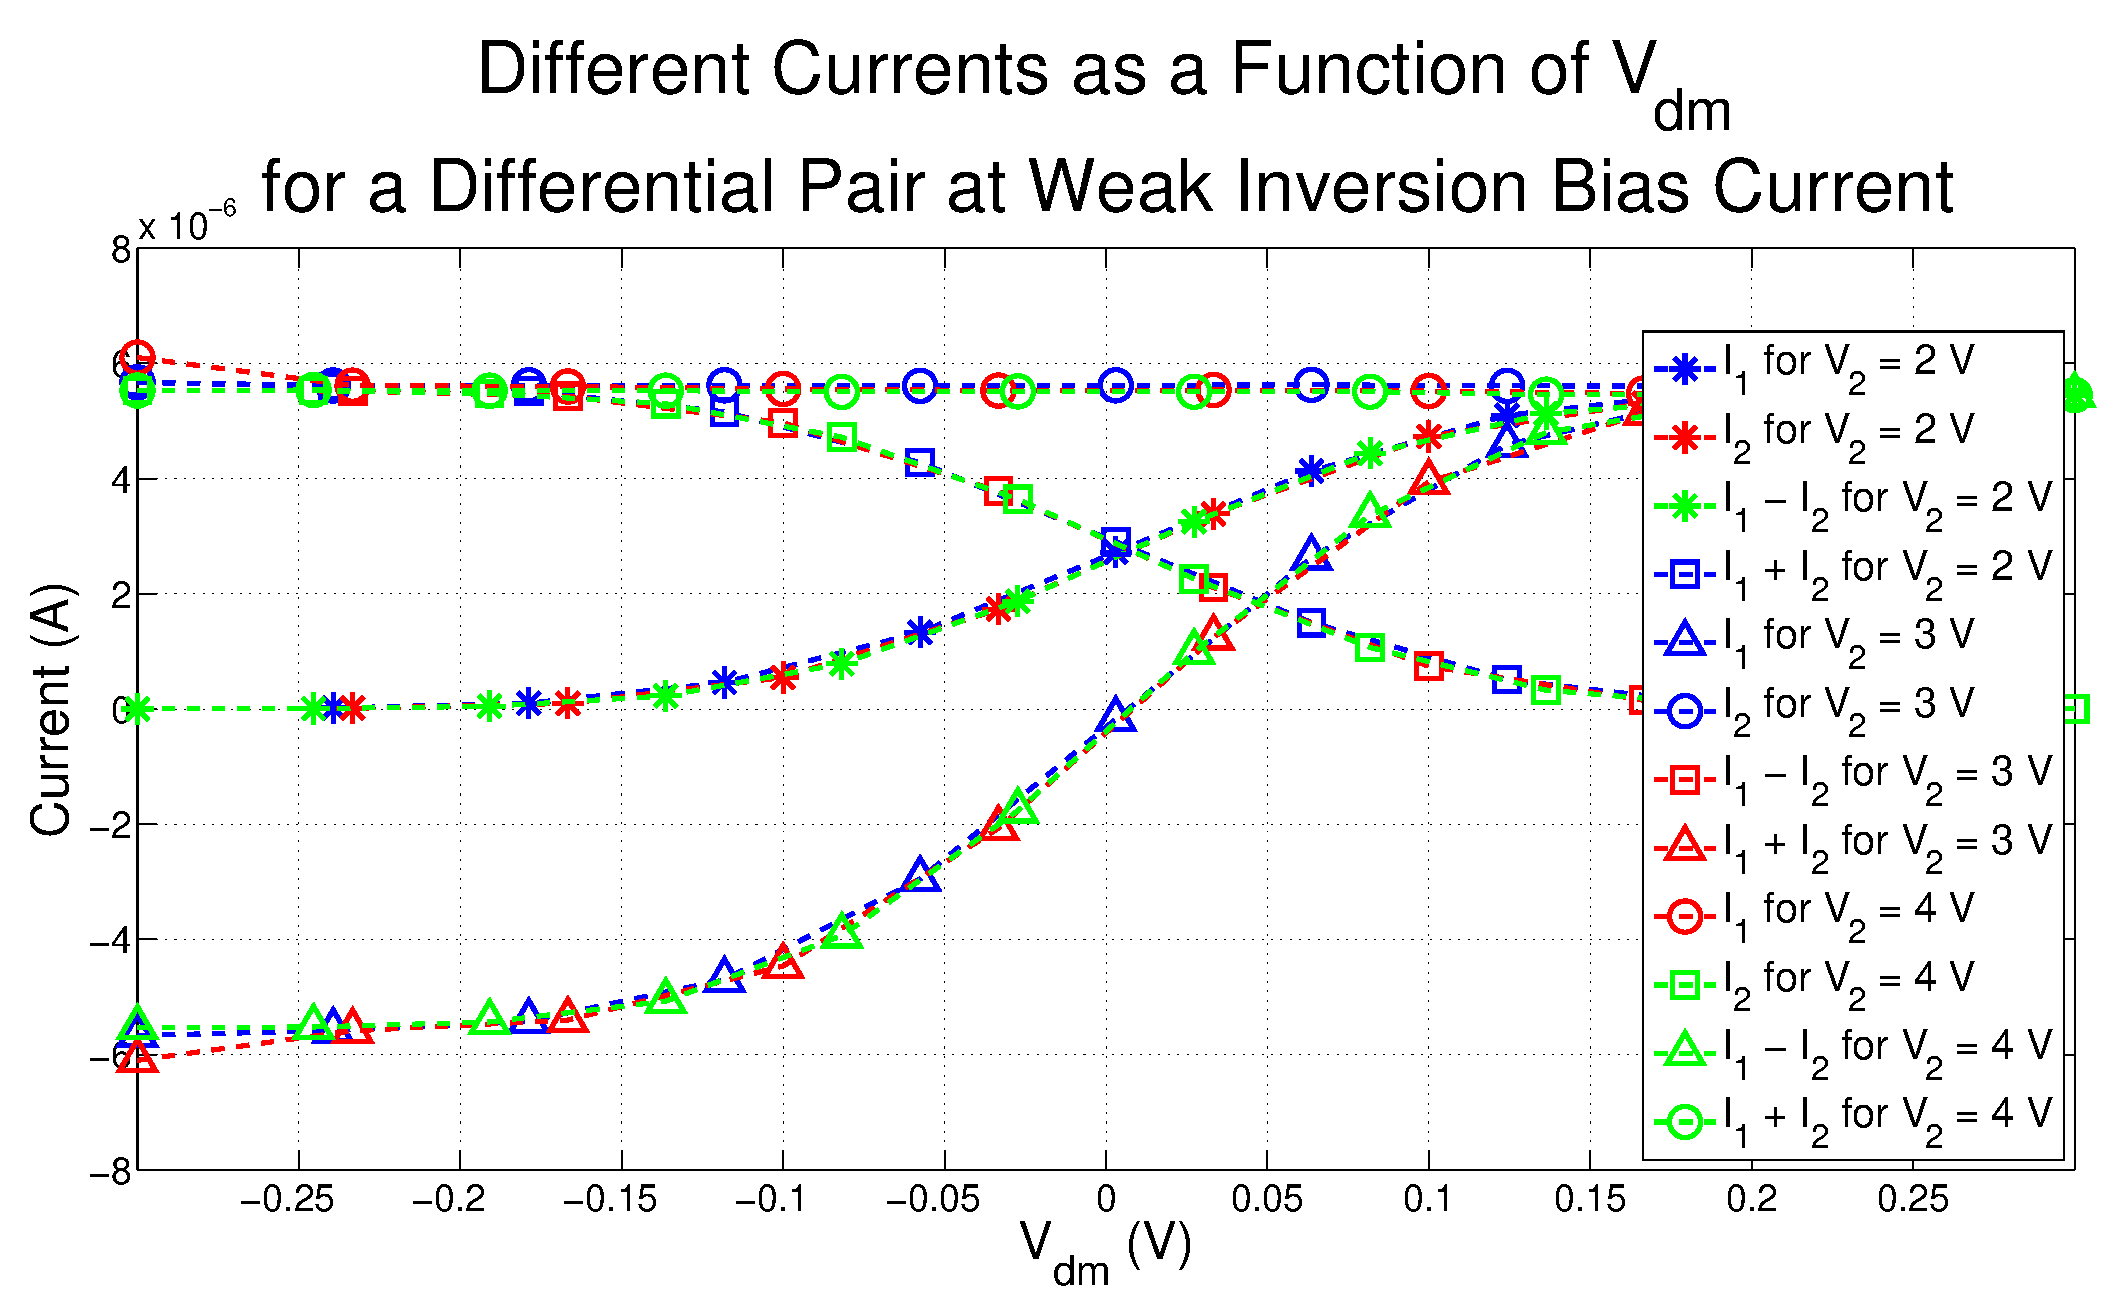
\includegraphics[width=\linewidth]{./Figures/AllCurrentsOneFigure}
\caption{The relationship between $I_1$ and $I_2$, shown through a range of different vales of $V_{DM}$ and \Vgb. The same information can is represented in Figure \ref{fig:AllCurrentsSubplot}, where it is more easily analyzed. }
\label{fig:AllCurrentsOneFigure }
\end{figure}

As seen below in Figure \ref{fig:AllCurrentsSubplot}, the current through $M_1$ and $M_2$ change significantly as $V_{DM}$ moves away from $0V$. As $V_{DM}$ increases, $I_1$ increases and $I_2$ decrease. For a decrease in $V_{DM}$, the opposite is true. 
As $V_2$ increases, the slope of the $I$, $V_{DM}$ relationship close to $0V$ increases in slope, further, the maximum current increases in magnitude with increased $V_2$. This difference can be seen most visibly in the plot of $I_1 -I_2$ as a function of $V_{DM}$, as $V_2$ increases, the slope close to the origin increases, and the maximum differential in current achieved is significantly larger, appearing to change linearly with increased $V_2$.

% Do these current–voltage characteristics change significantly as
% V2 changes? Also include a plot showing the common-source node voltage, V , as a function
% of V1
% −V2 for all three values of V2. How does the value of V change as V1 goes from below
% V2 to above it?

% In your report, include a single plot showing I1, I2, I1−I2, and I1+I2, as a function of V1−V2 for all three values of V2 that you used. Do these current–voltage characteristics change significantly asV2 changes? 




\begin{figure}[H]
\centering
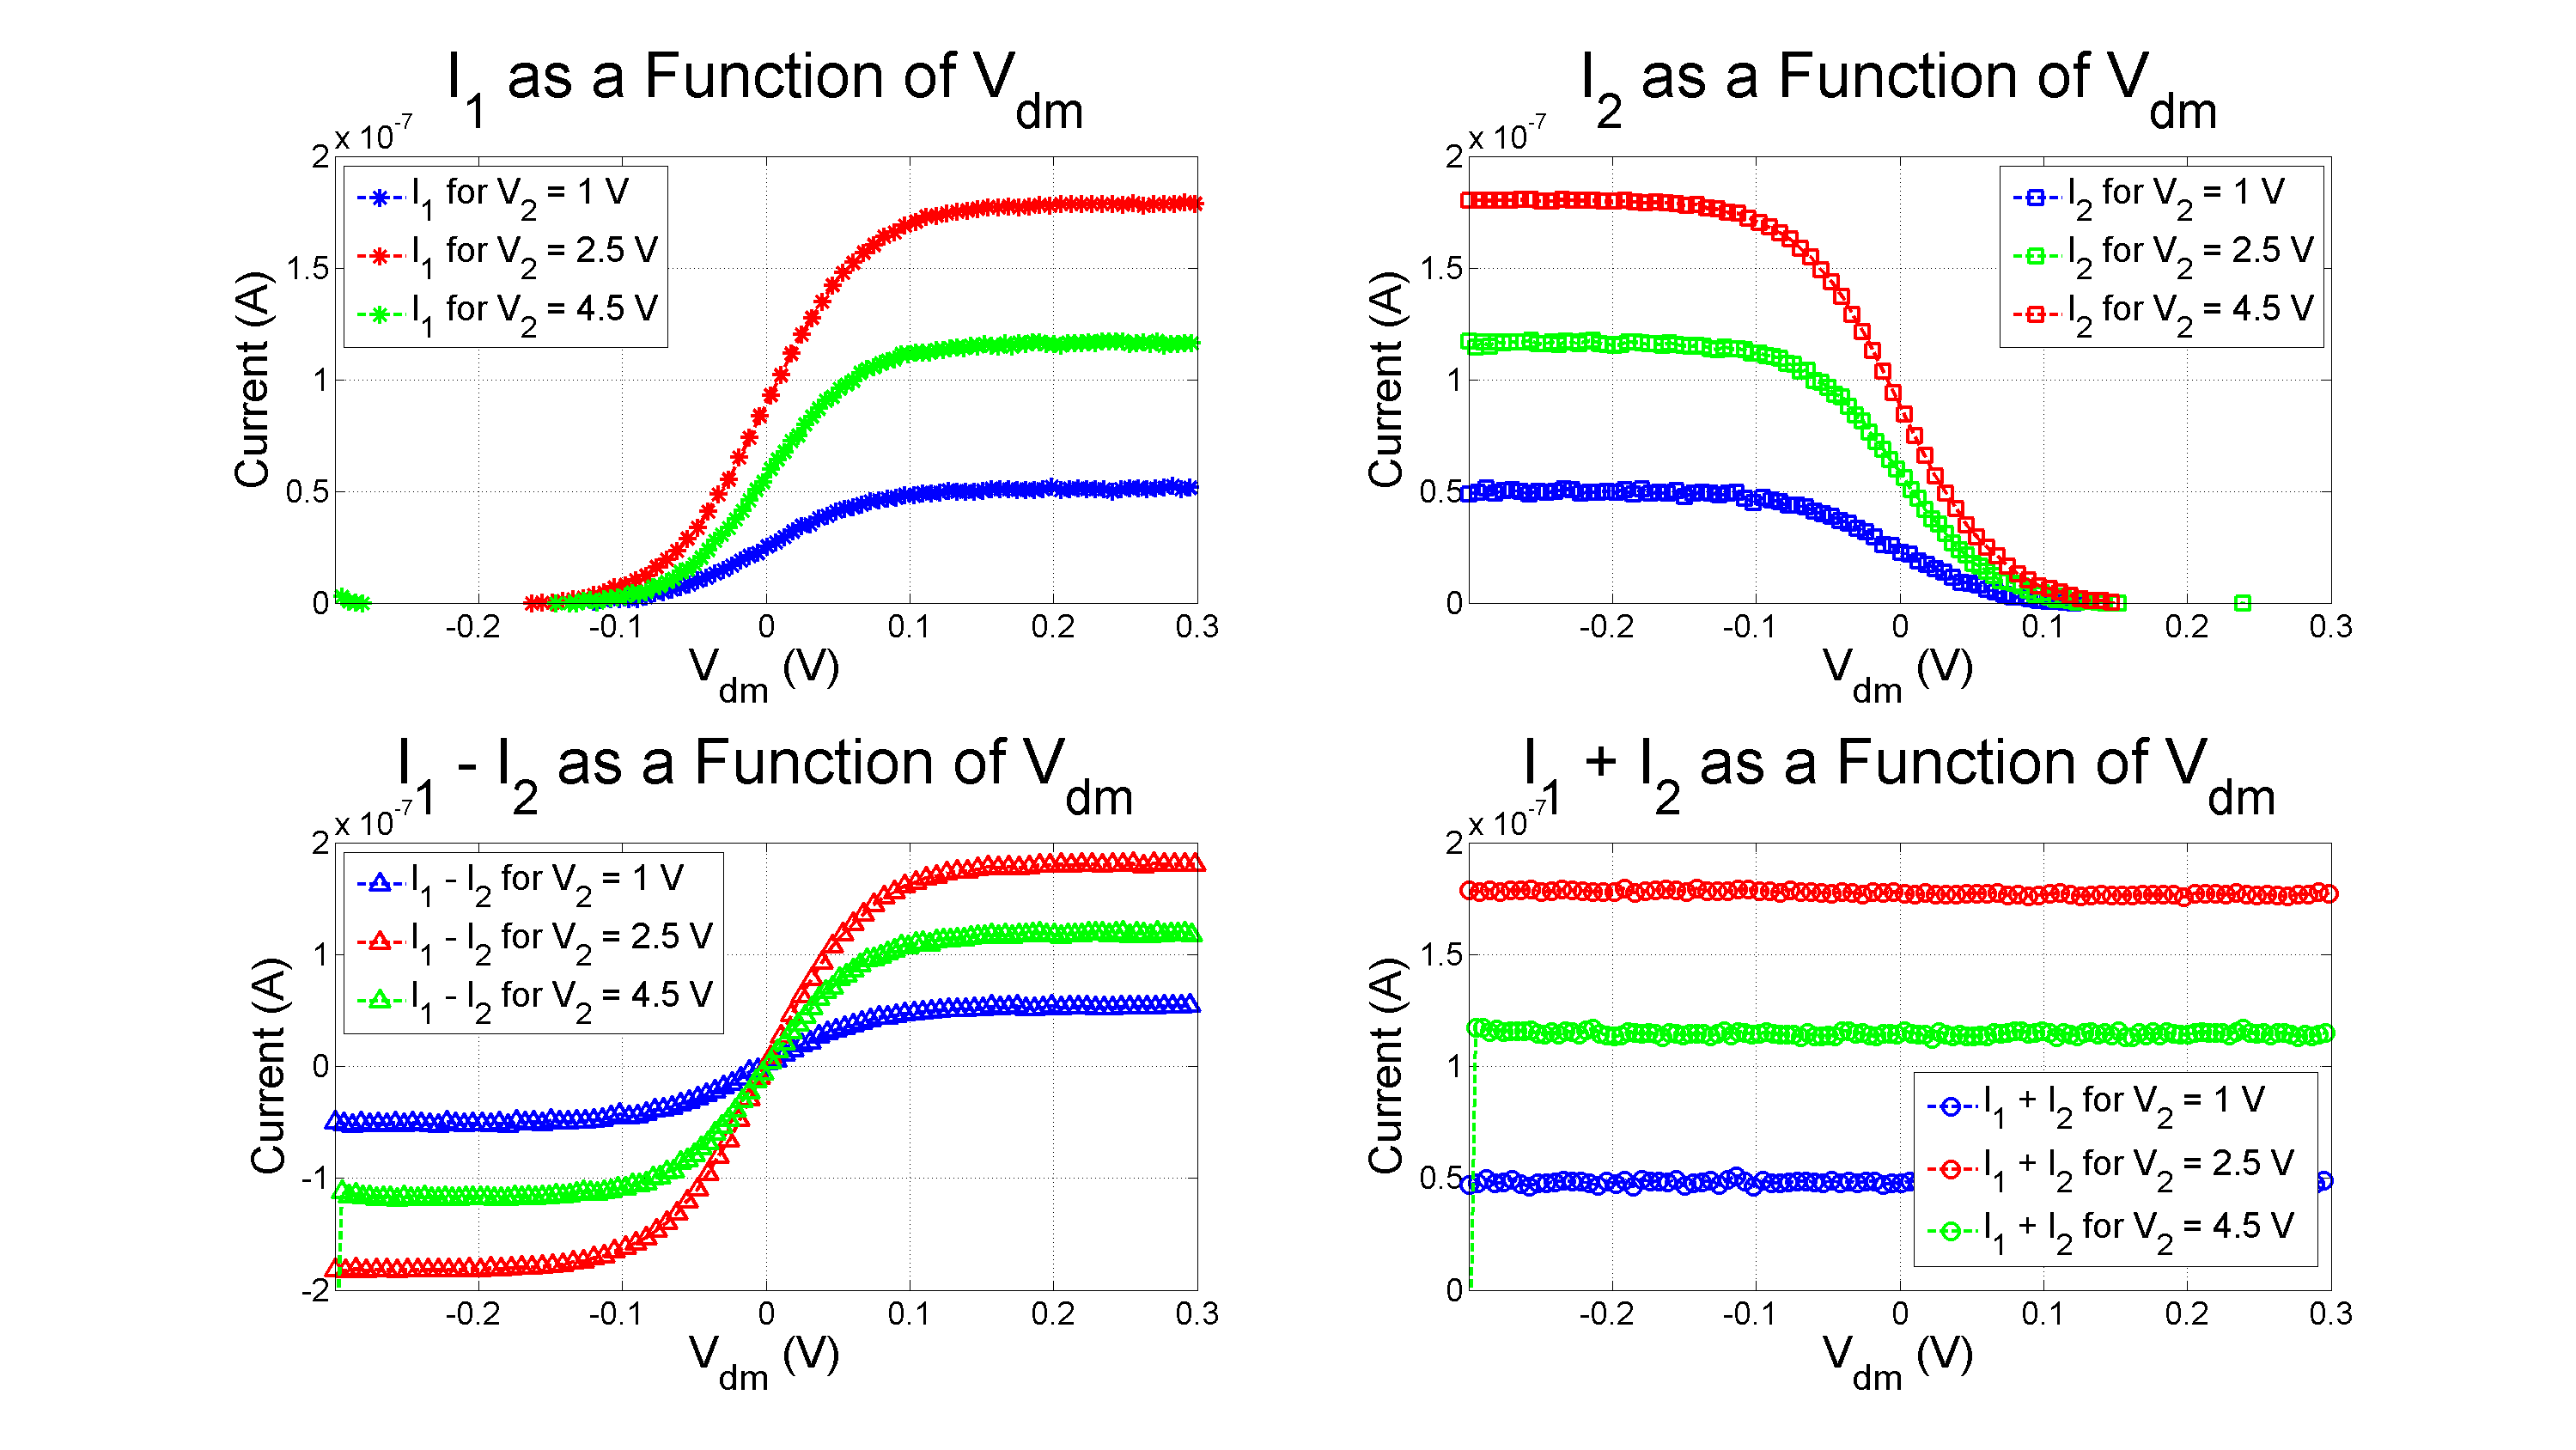
\includegraphics[width=\linewidth]{./Figures/AllCurrentsSubplot}
\caption{A more readable representation Figure \ref{fig:AllCurrentsOneFigure}}
\label{fig:AllCurrentsSubplot}
\end{figure}

\section*{Common-source Node voltage}
% Also include a plot showing the common-source node voltage, V , as a functionof V1−V2 for all three values of V2. How does the value of V change as V1 goes from below V2 to above it?

From the pre-lab, we expect the common-source node voltage $V$ to operate according to the following equation:

\begin{equation}
V = \kappa (\textrm{max}(V_1,V_2) - V_b)
\label{eq:nodevoltageeq}
\end{equation}

In this first experiment, we set \Vtwo while adjusting \Vone, so we expect a graph of the $V$ as a function of \Vdm to be constant when $V_{dm} < 0$ and to follow \Vone when $V{dm} > 0$. We in fact see this in figure \ref{fig:nodevoltageWI}, where $V$ is plotted as a function of \Vdm for three values of \Vtwo.

\begin{figure}[H]
\centering
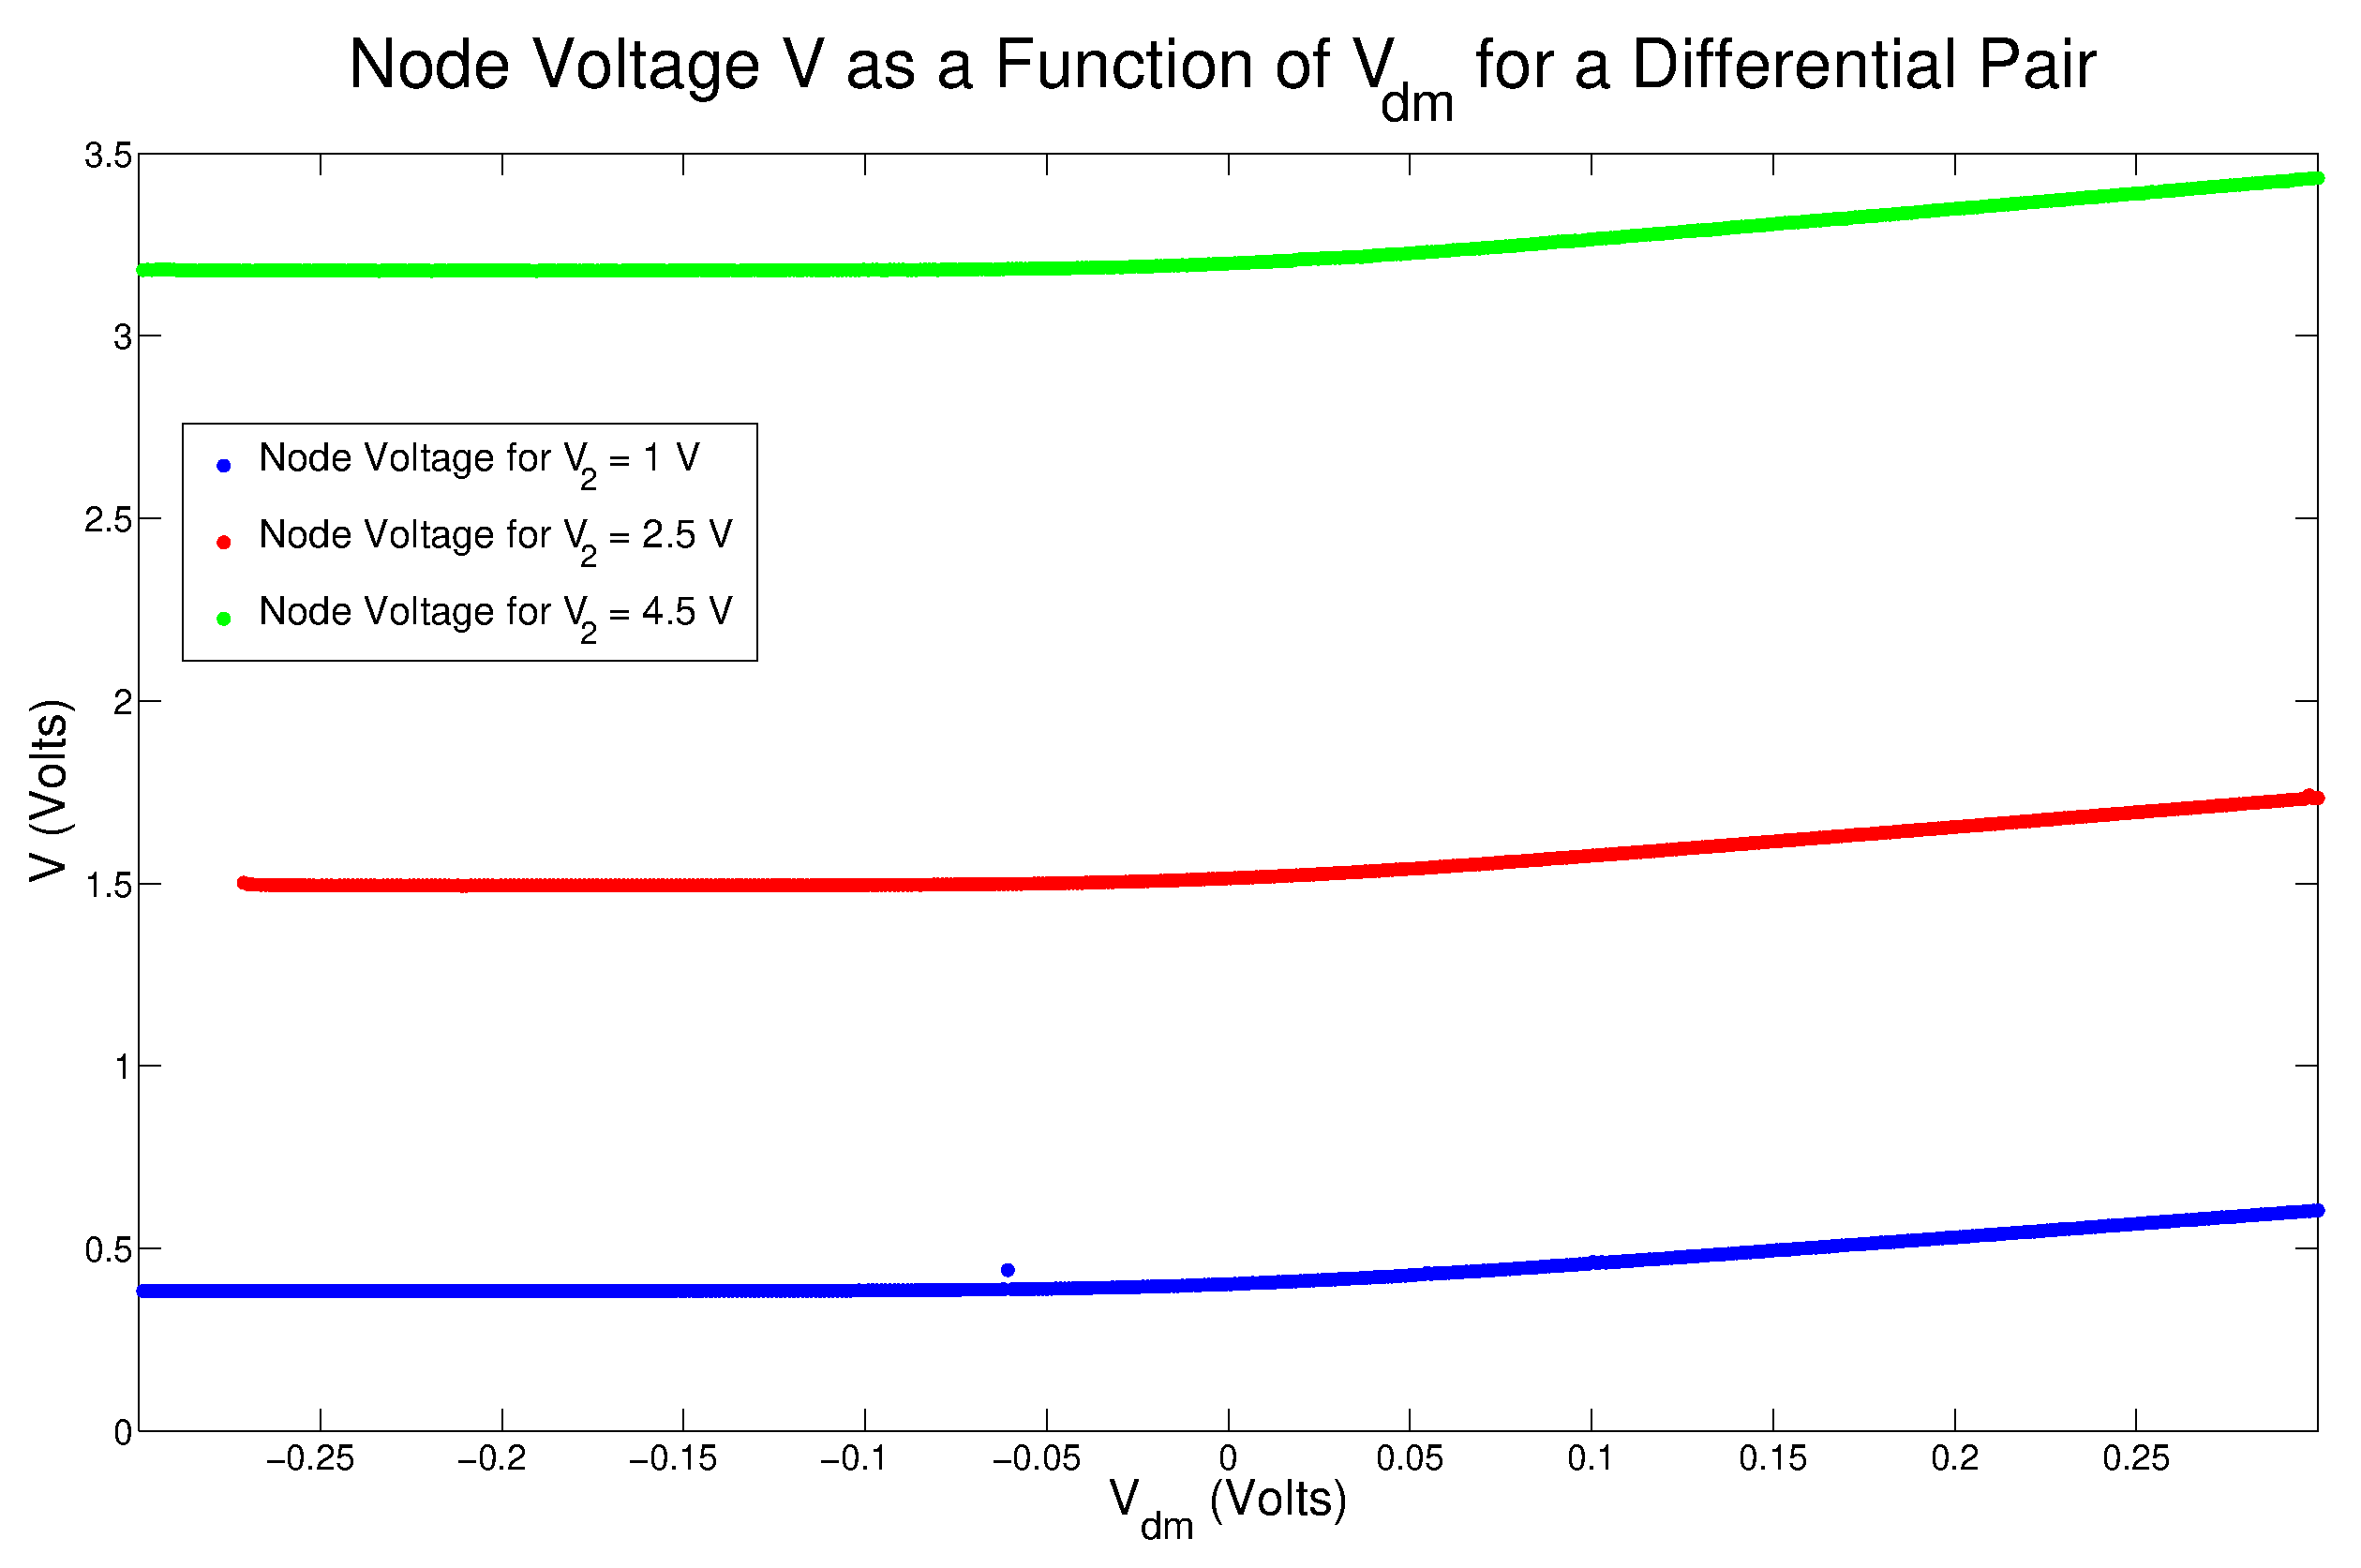
\includegraphics[width=\linewidth]{./Figures/NodeVoltageWeakInversion.eps}
\caption{Node voltage as a function of the differential mode voltage. Governed by equation \ref{eq:nodevoltageeq}, we see $V$ follow \Vtwo (which was constant for each separate experiment) when $V_{dm} < 0$ and follow \Vone when $V_{dm} > 0$.}
\label{fig:nodevoltageWI}
\end{figure}

In figure \ref{fig:nodevoltageWI}, when $V_{dm} < 0$, we see that $V$ is set to a constant value, and when $V_{dm} > 0$, we see it rise almost linearly. The behavior when $V_{dm} < 0$ is explained by $V$ following a function of \Vtwo, specifically:

\begin{equation*}
    V = \kappa V_2 - V_b.
\end{equation*}

As \Vtwo is constant in these experiments, the value of $V$ remains constant. When $V_{dm} > 0$, we see $V$ increase linearly, which is explain by the fact that we were adjusting \Vone linearly, and $V$ follows \Vone.

To double check that equation \ref{eq:nodevoltageeq} well-described the behavior of $V$ as a function of \Vdm, we plugged in values of \Vone, \Vtwo and \Vb into equation \ref{eq:nodevoltageeq} and compares the values of $\kappa$. 

% For each of the three values of V2 that you used, fit a straight line to the plot of I1−I2 asa function of V1− V2 around the region where V1~ V2 (i.e., where V1−V2~ 0). The slope of this line is approximately equal to the (incremental) differential-mode transconductancegain of the differential pair, which is formally given by ... Does the value of the differential-mode transconductance gain change significantly as V2 changes?

\begin{figure}[H]
\centering
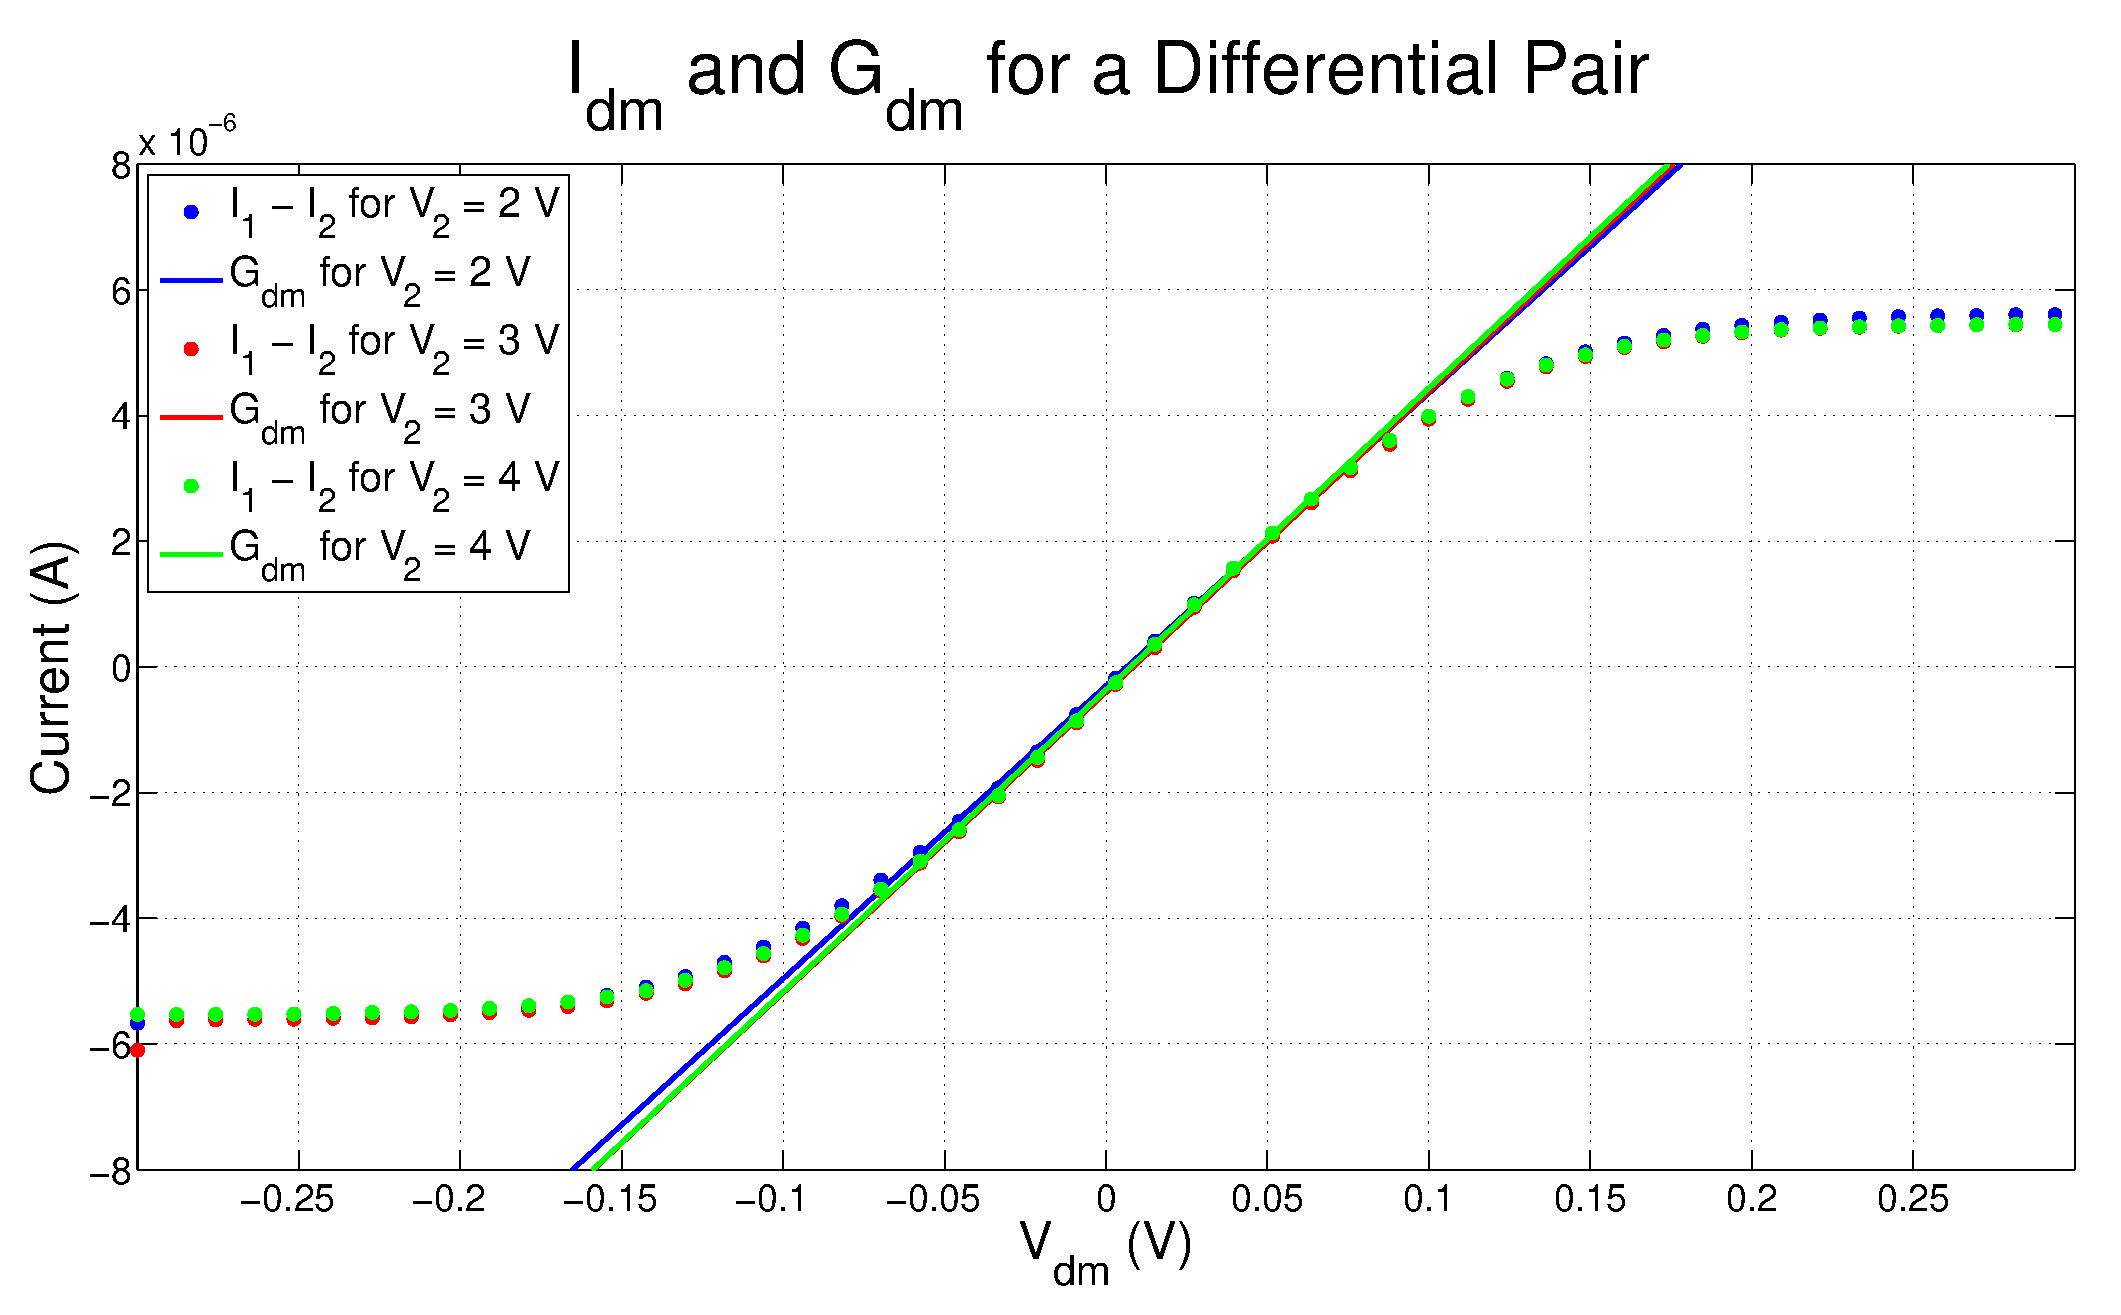
\includegraphics[width=\linewidth]{./Figures/Gdm.eps}
\caption{Gdm changes!!}
\label{fig:gdm}
\end{figure}

\begin{table}[h]
\begin{center}
    \begin{tabular}{ l | l  }
        V2 (Volts) & $G_{dm} (\Omega^{-1})$ \\
        \hline
        1 & $6.7086 \times 10^{-7}$ \\
        2.5 & $2.4470 \times 10^{-6}$ \\
        4.5 & $1.6894 \times 10^{-6}$ \\
        \label{tb:gdm}
    \end{tabular}
\end{center}
\end{table}


% Now, set the bias voltage, Vb, so that the bias current is above threshold. For a singlevalue of V2 that is far enough away from the power supply rail to keep the bias transistor saturated, perform these same measurements. You might want to increase slightly the rangeover which you sweep V1− V2 for these measurements. Make plot similar to the ones thatyou made for the lower bias current. How does the behavior of the circuit change as the biascurrent changes from weak or moderate inversion to strong inversion?

%AllCurrentsStrongInversion

\begin{figure}[H]
\centering
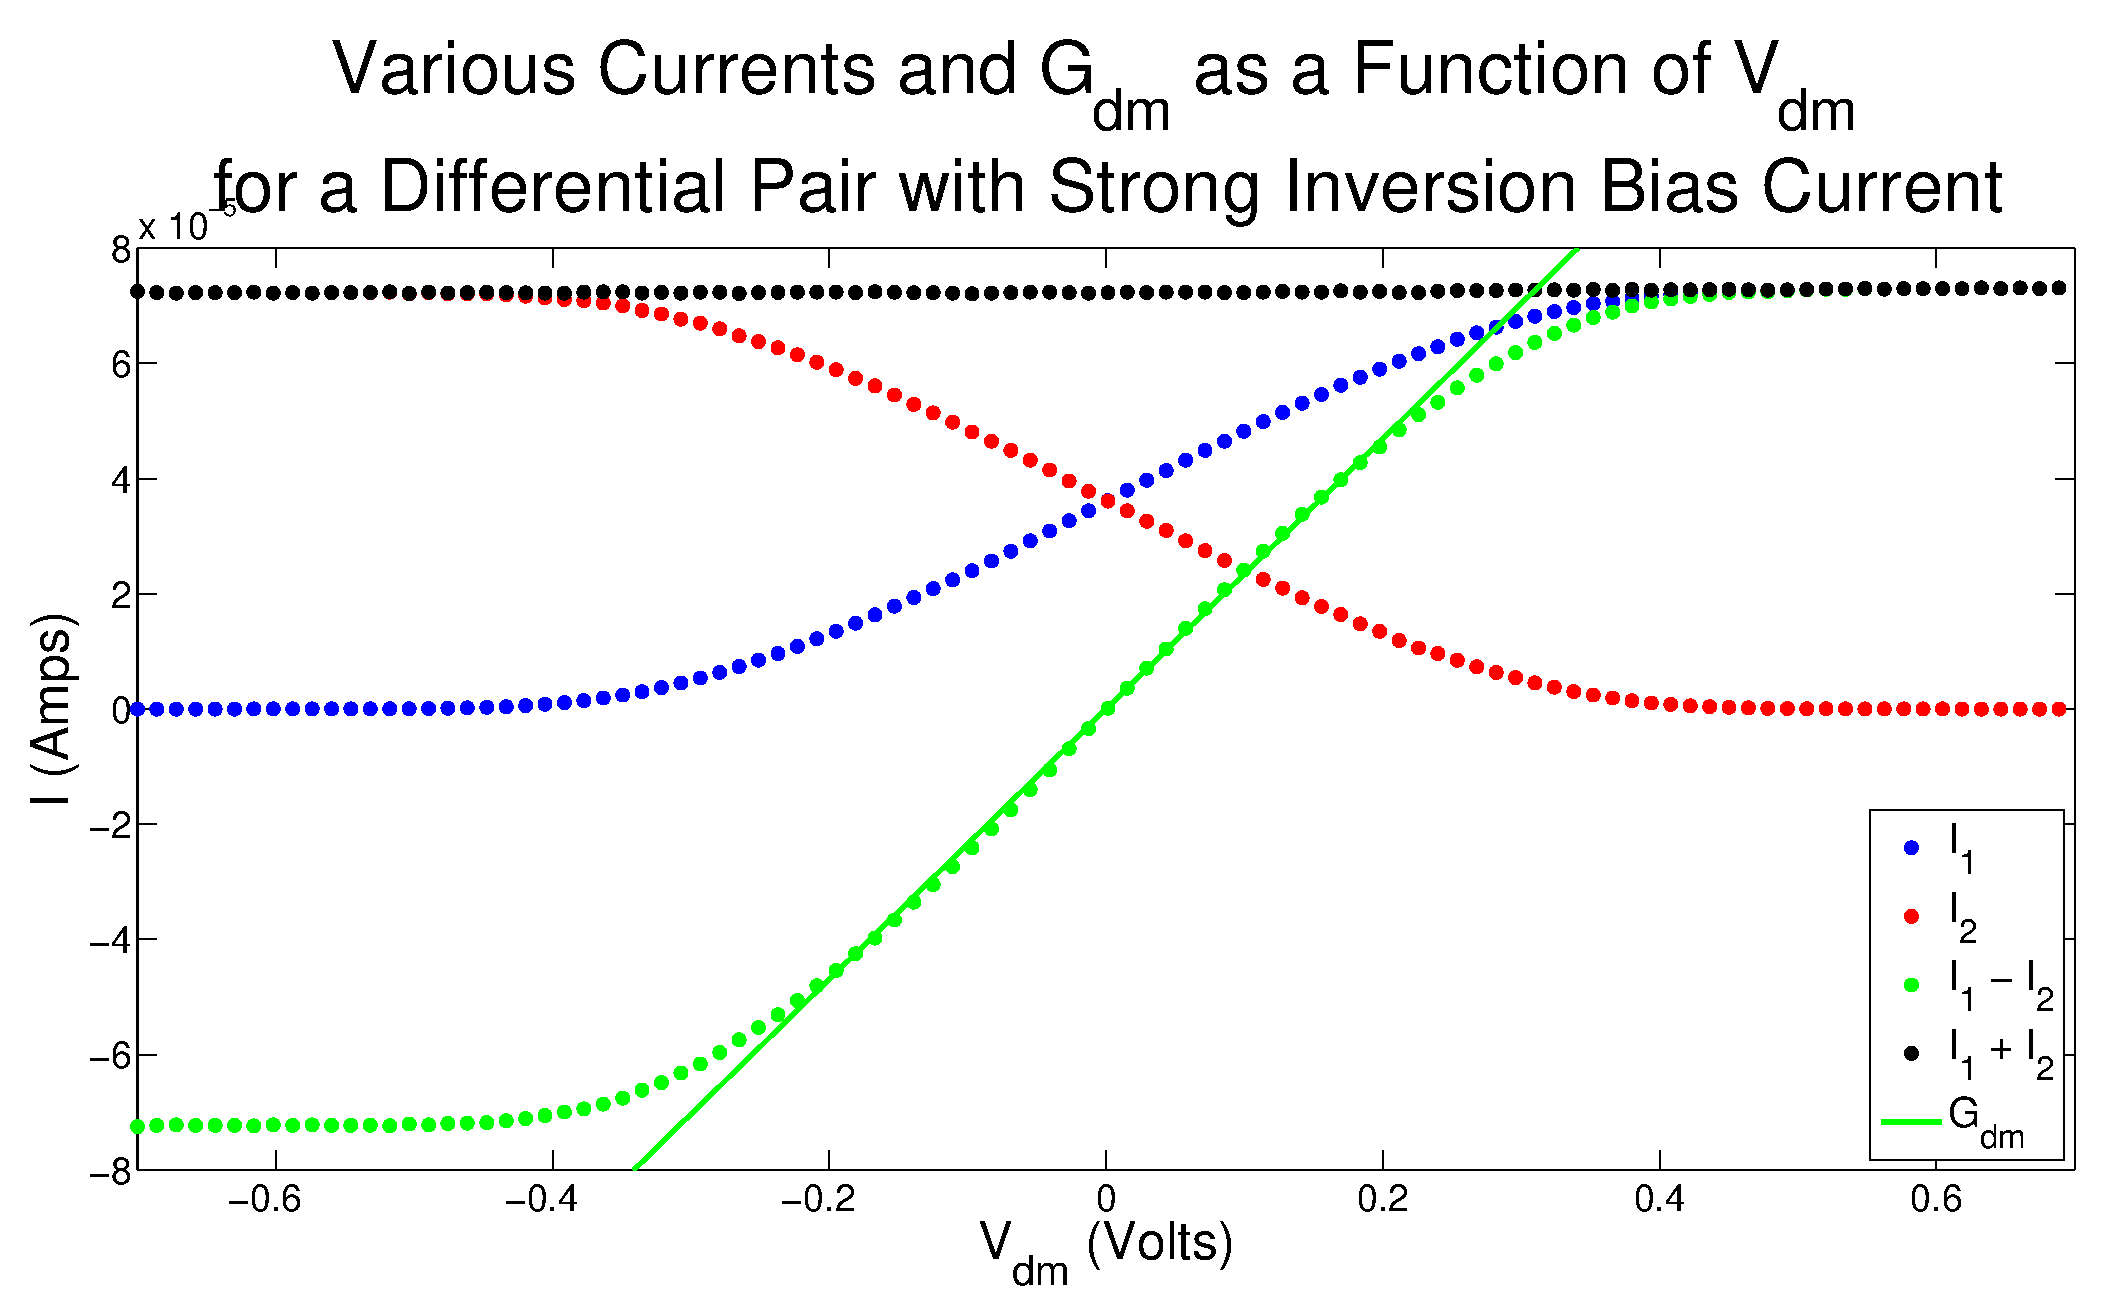
\includegraphics[width=\linewidth]{./Figures/AllCurrentsStrongInversion.eps}
\caption{Something descriptive. }
\label{fig:AllCurrentsStrongInversion }
\end{figure}

%NoldeVoltageStrongInversion

\begin{figure}[H]
\centering
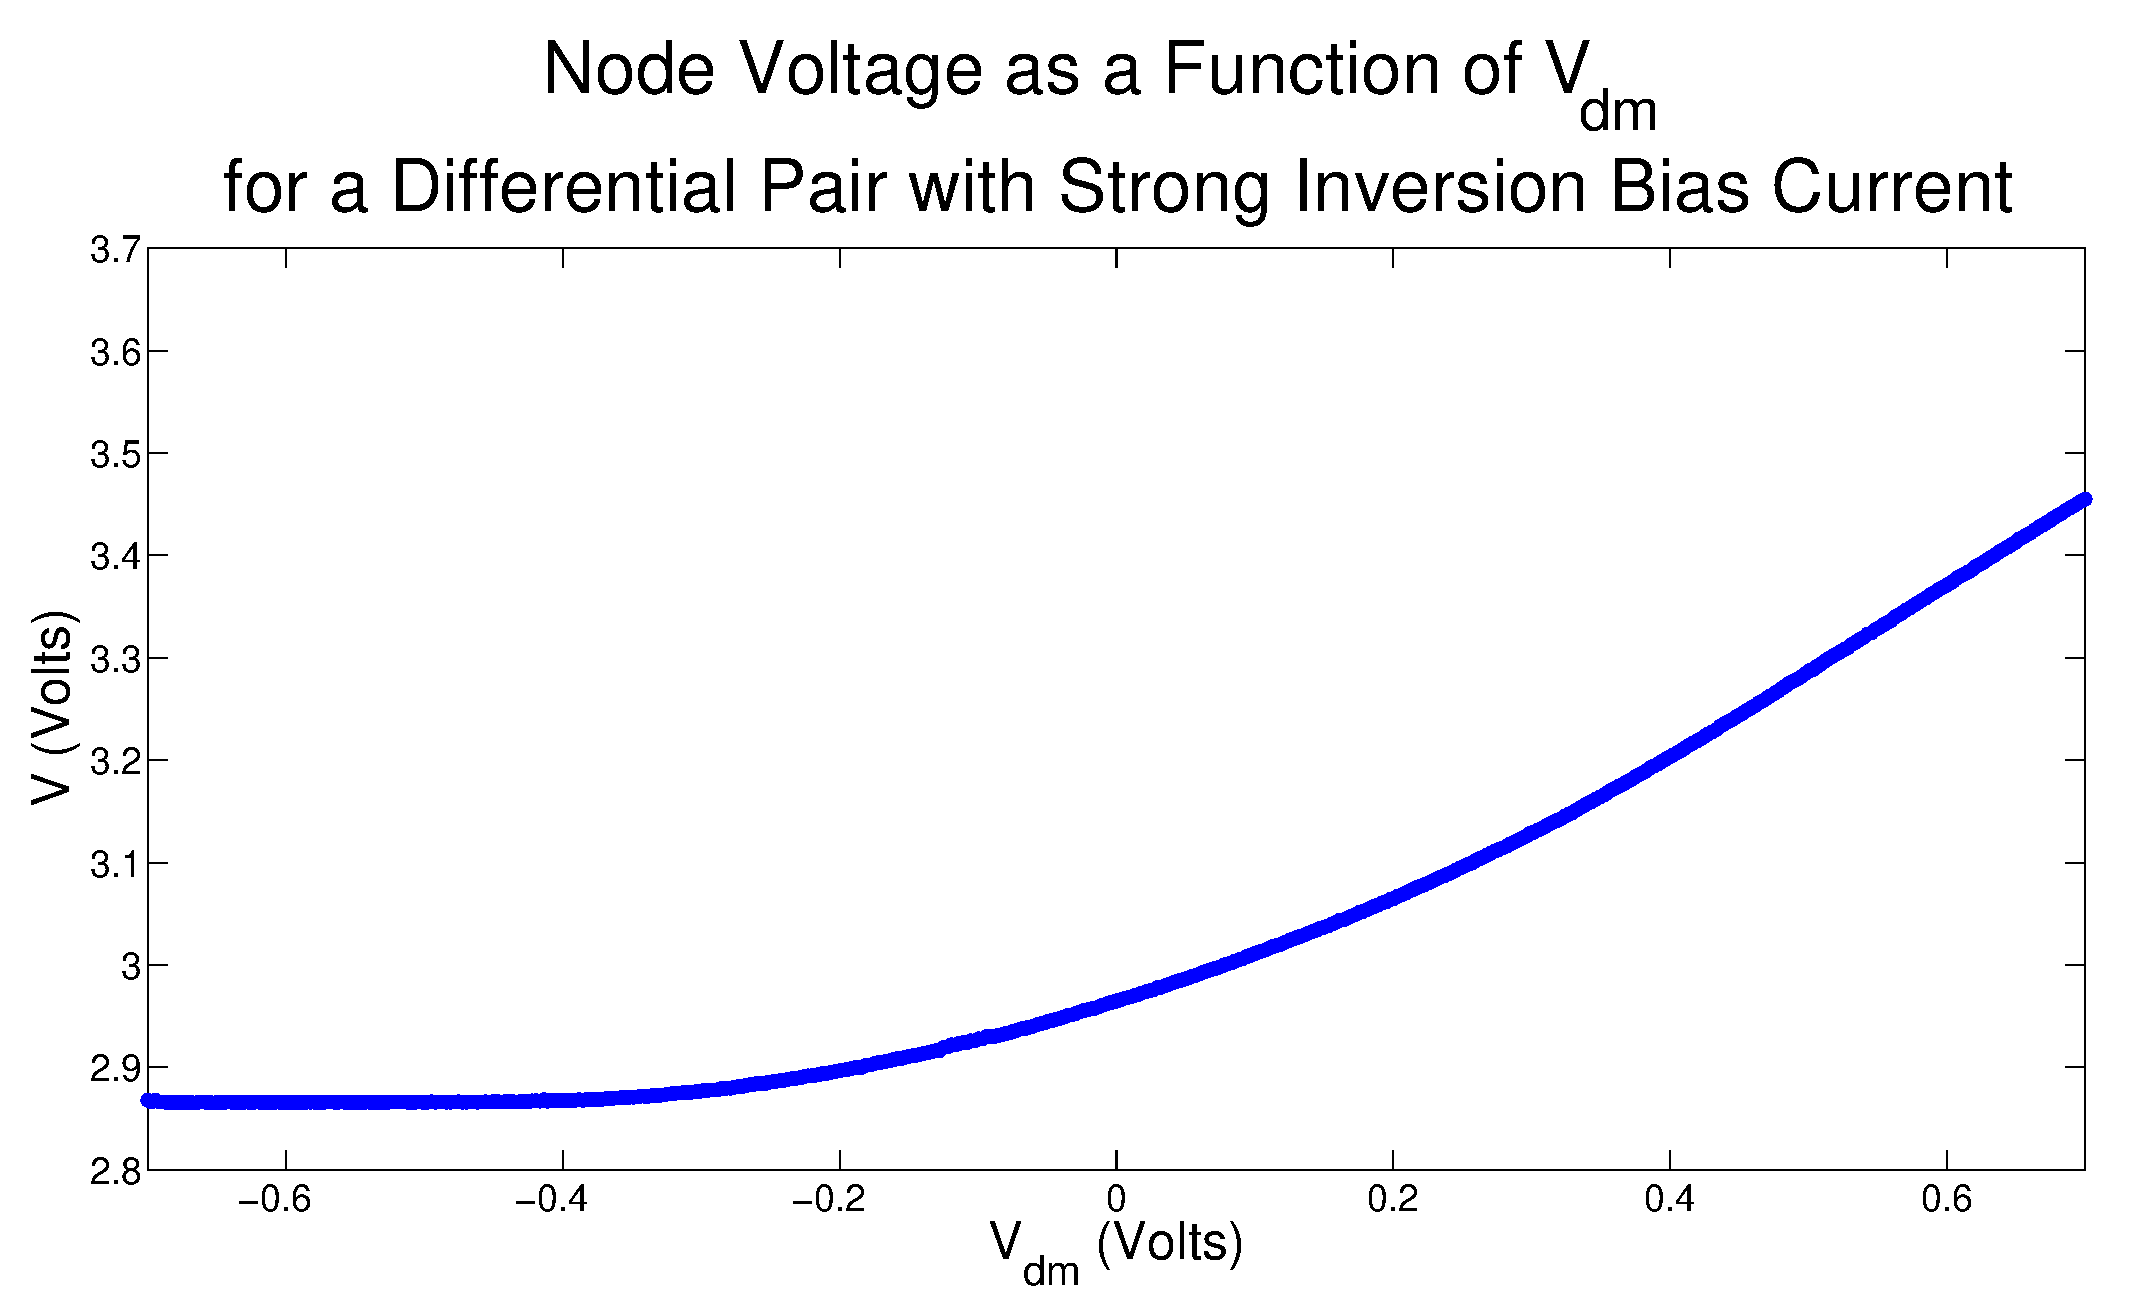
\includegraphics[width=\linewidth]{./Figures/NodeVoltageStrongInversion.eps}
\caption{The node voltage follows the larger voltage!!}
\label{fig:nodevoltageSI}
\end{figure}


\end{document}